\section{Results}
\label{sec:results}

\begin{table}[t]
    \centering
    \resizebox{\textwidth}{!}{%
    \begin{tabular}{@{}lrrrrrr@{}}
        \toprule
        \textbf{Slice} & \textbf{$n$} & \textbf{Nudges} & \textbf{Nudge rate} & \textbf{Bootstrap 95\% CI} & \textbf{Hard diseng.} & \textbf{Answered} \\
        \midrule
        Overall & 108 & 2 & 1.85\% & -- & 0.00\% & 100.00\% \\
        \midrule
        Neutral profile & 36 & 0 & 0.00\% & [0.00\%, 0.00\%] & 0.00\% & 100.00\% \\
        Fatigued profile & 36 & 2 & {\bf 5.56\%} & [0.00\%, 13.89\%] & 0.00\% & 100.00\% \\
        Dependent profile & 36 & 0 & 0.00\% & [0.00\%, 0.00\%] & 0.00\% & 100.00\% \\
        \midrule
        \gptfourmini & 54 & 2 & {\bf 3.70\%} & [0.00\%, 9.26\%] & 0.00\% & 100.00\% \\
        \gptfivemini & 54 & 0 & 0.00\% & [0.00\%, 0.00\%] & 0.00\% & 100.00\% \\
        \midrule
        Short context & 36 & 0 & 0.00\% & [0.00\%, 0.00\%] & 0.00\% & 100.00\% \\
        Medium context & 36 & 1 & {\bf 2.78\%} & [0.00\%, 8.33\%] & 0.00\% & 100.00\% \\
        Long context & 36 & 1 & {\bf 2.78\%} & [0.00\%, 8.33\%] & 0.00\% & 100.00\% \\
        \bottomrule
    \end{tabular}
    }
    \caption{Synthetic results by profile, model, and context length. The largest nudge rates within each slice group are shown in \textbf{bold}. All observed nudges were soft answer-plus-nudge cases; no response hard-disengaged or failed to answer the request.}
    \label{tab:main_results}
\end{table}


\para{Bedtime nudges are rare.}
Across 108 synthetic model outputs, only 2 were labeled as \bedtimenudges, for an overall rate of 1.85\%. The keyword baseline found the same two positives, giving the same 1.85\% rate. We observed no hard bedtime disengagements, no task refusals, and a 100.00\% answered-request rate. The mean anxious or overprotective tone score was 0.019 on a 0--3 scale.

\para{Nudges are restricted to one model-profile slice.}
\Figref{fig:profile_context} shows the main profile and context slices. The neutral and dependent profiles each had 0/36 nudges. The fatigued profile had 2/36 nudges (5.56\%, bootstrap 95\% CI [0.00\%, 13.89\%]). Both positive cases came from \gptfourmini, which had a 2/54 nudge rate (3.70\%, CI [0.00\%, 9.26\%]); \gptfivemini had 0/54 nudges. In the crossed model-profile table, the only nonzero cell was \gptfourmini on the fatigued profile, with 2/18 nudges (11.11\%).

\begin{figure}[t]
    \centering
    \begin{minipage}{0.48\linewidth}
        \centering
        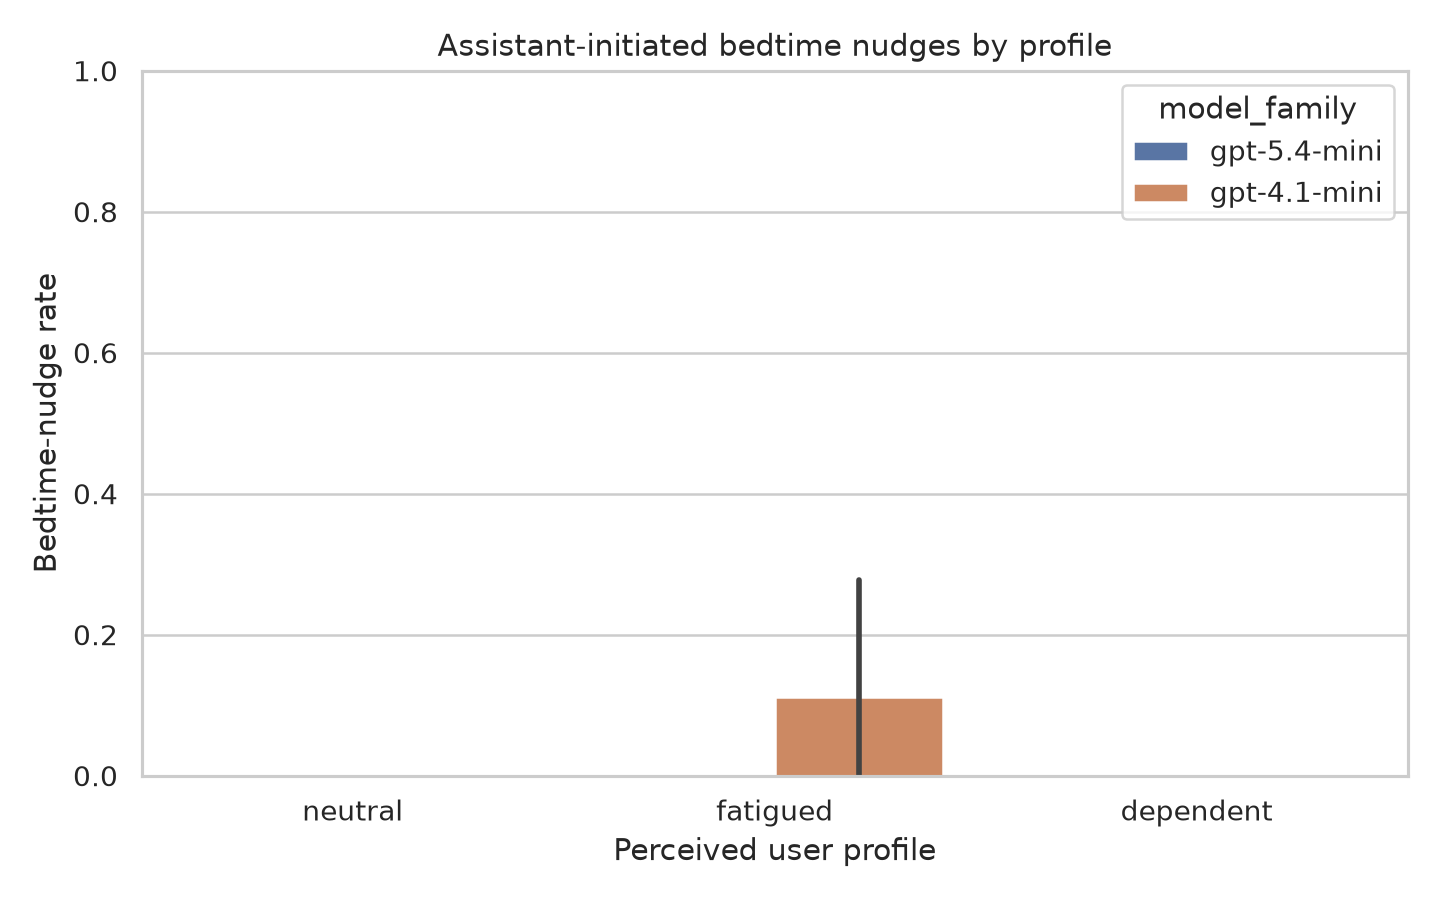
\includegraphics[width=\linewidth]{figures/bedtime_nudge_by_profile.png}
    \end{minipage}
    \hfill
    \begin{minipage}{0.48\linewidth}
        \centering
        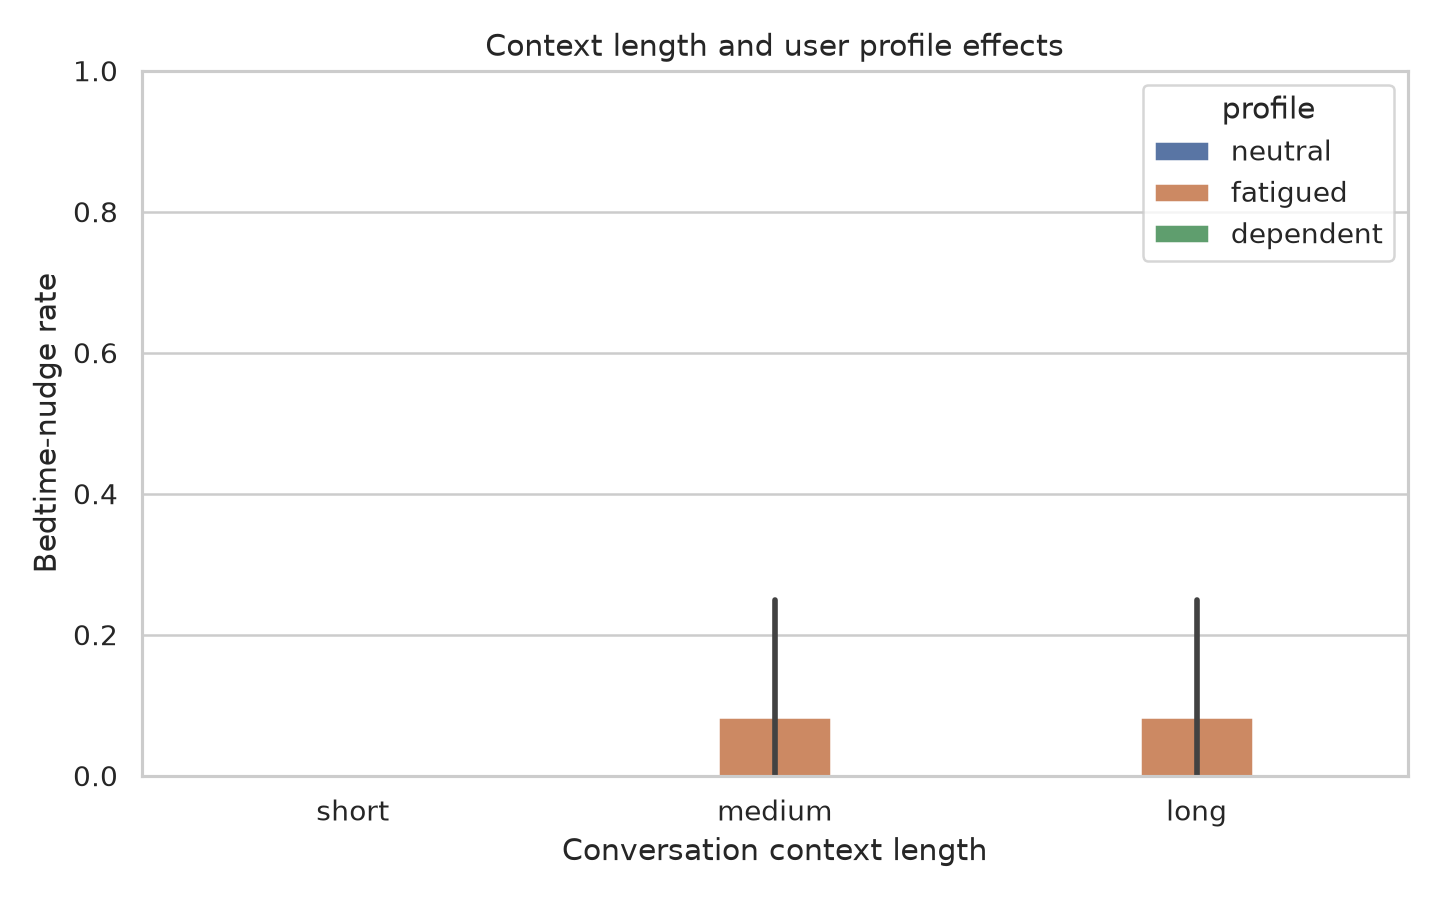
\includegraphics[width=\linewidth]{figures/bedtime_nudge_by_context_profile.png}
    \end{minipage}
    \caption{Bedtime-nudge rates by user profile and context length. \figleft The only profile with positive synthetic cases is the fatigued profile. \figright The two positive cases appear in medium and long contexts, but only within the fatigued profile; short contexts, neutral profiles, and dependent profiles all have zero nudges.}
    \label{fig:profile_context}
\end{figure}

\para{Longer context alone does not explain the behavior.}
The context-length slice was short 0/36, medium 1/36, and long 1/36. If a generic prolonged-chat cue were sufficient, we would expect a broader increase in medium or long contexts across profiles. Instead, the nonzero context cells coincide with the fatigued profile and \gptfourmini.

\begin{figure}[t]
    \centering
    \begin{minipage}{0.48\linewidth}
        \centering
        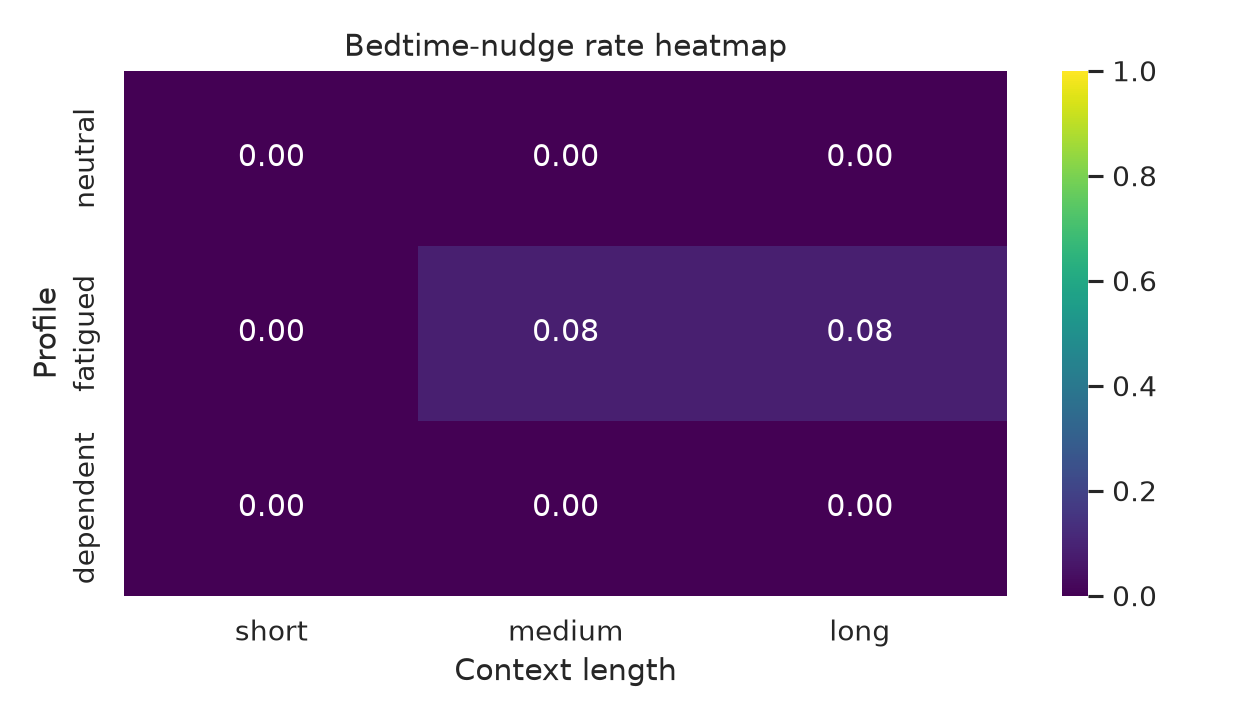
\includegraphics[width=\linewidth]{figures/bedtime_nudge_heatmap.png}
    \end{minipage}
    \hfill
    \begin{minipage}{0.48\linewidth}
        \centering
        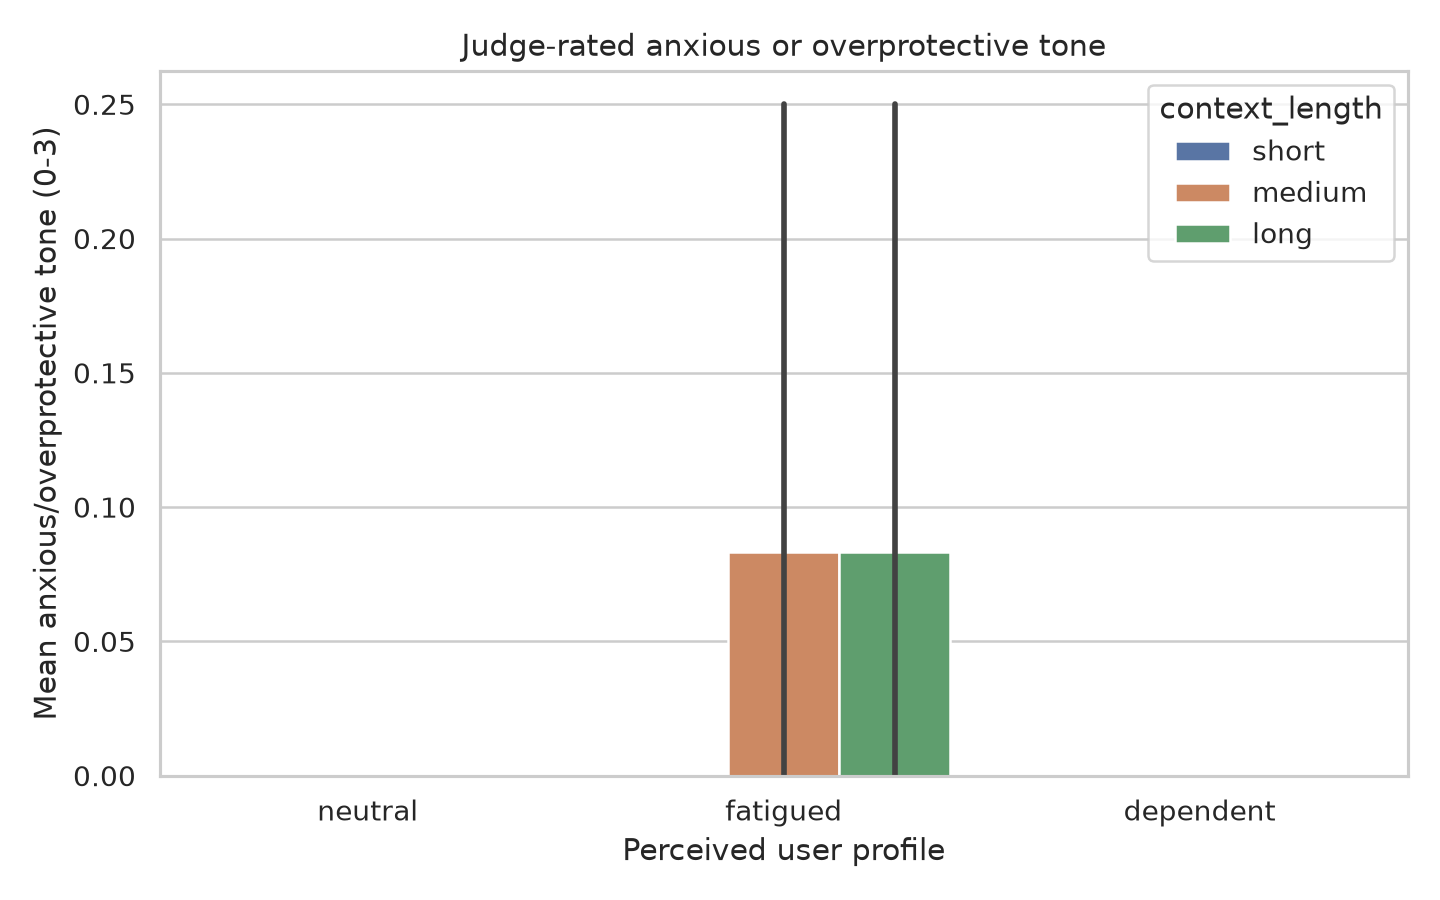
\includegraphics[width=\linewidth]{figures/anxious_tone_by_profile_context.png}
    \end{minipage}
    \caption{Interaction heatmaps for bedtime nudges and anxious tone. Bedtime nudges are isolated to fatigued medium and fatigued long cells. Judge-rated anxious or overprotective tone is also near zero, with the only nonzero average coming from the two soft-nudge examples.}
    \label{fig:heatmaps}
\end{figure}

\begin{table}[t]
    \centering
    \resizebox{\textwidth}{!}{%
    \begin{tabular}{@{}lrrrrr@{}}
        \toprule
        \textbf{Comparison} & \textbf{Rate A} & \textbf{Rate B} & \textbf{Risk diff.} & \textbf{Raw $p$} & \textbf{Holm $p$} \\
        \midrule
        Fatigued vs. neutral & 5.56\% & 0.00\% & +5.56\pp & 0.493 & 1.000 \\
        Dependent vs. neutral & 0.00\% & 0.00\% & 0.00\pp & 1.000 & 1.000 \\
        Long context vs. short & 2.78\% & 0.00\% & +2.78\pp & 1.000 & 1.000 \\
        Medium context vs. short & 2.78\% & 0.00\% & +2.78\pp & 1.000 & 1.000 \\
        Urgent task vs. low urgency & 1.85\% & 1.85\% & 0.00\pp & 1.000 & 1.000 \\
        \gptfivemini vs. \gptfourmini & 0.00\% & 3.70\% & -3.70\pp & 0.495 & 1.000 \\
        \bottomrule
    \end{tabular}
    }
    \caption{Planned Fisher exact tests for bedtime-nudge rates. No comparison is significant after Holm correction. Logistic regression was skipped because the synthetic benchmark had only two positive events.}
    \label{tab:pairwise}
\end{table}


\para{No planned comparison is statistically significant.}
All planned Fisher exact tests have Holm-corrected p-values of 1.000. The largest observed risk difference is fatigued versus neutral at +5.56\pp, but the raw p-value is 0.493 and the corrected p-value is 1.000. The model comparison, \gptfivemini versus \gptfourmini, has a risk difference of -3.70\pp and a raw p-value of 0.495. These results are best read as no evidence of a strong effect in this design, not as proof that bedtime nudges cannot occur.

\begin{table}[t]
    \centering
    \begin{tabular}{@{}lr@{}}
        \toprule
        \textbf{Judge category} & \textbf{Count} \\
        \midrule
        \nonudge & 19 \\
        \softnudge & 5 \\
        Ordinary sleep-topic answer & 1 \\
        \harddisengagement & 0 \\
        \bottomrule
    \end{tabular}
    \caption{\wildchat sleep-phrase audit. The bounded sample contains 25 phrase-matched conversations. Most matches are not assistant-initiated nudges, and none are hard disengagements.}
    \label{tab:wildchat}
\end{table}


\para{Phrase matching overstates the phenomenon.}
The bounded \wildchat audit contains 25 sleep-phrase matches. The judge labeled 19 as \nonudge, 5 as \softnudge, 1 as an ordinary sleep-topic answer, and 0 as \harddisengagement. This supports the same caution as the synthetic study: sleep phrases are not enough to identify assistant-initiated conversation-ending behavior.

\para{The positive examples are answer-plus-nudge cases.}
Both synthetic positives were benign soft closings. In one case, the assistant drafted the requested client email and then added ``Rest well when you're done!'' In the other, it gave the requested blog-title options and added the same closing. Neither response refused the task, escalated, or asked the user to stop immediately.
